\section{Choice of Input Data}

Selecting the optimal form of input data is a paramount initial step in designing \glspl{dnn}.
This choice is influenced by the data's capacity to efficiently encode the coveted information, ensuring that the model
can effectively learn and generalize from the input data, without overfitting on irrelevant features.


\subsection{Evaluation of Input Data Forms}

Various forms of input data were considered, assessing their potential in effectively conveying information pertinent to
model order estimation:

\textbf{Measurement Matrix \( \bfm{X} \):}
The sub-sampled measurement matrix \( \bfm{X} \in \mathbb{R}^{M \times L} \) contains the IQ samples of the
individual subarrays, each column consisting of \( L \) complex data points. \\
This form of input data offers a direct signal representation but entails the highest dispersion of the sought-after
model order information.

A system with \( M = 9 \) antennas, \( L = 3 \) RF chains, and \( K = 100 \) snapshots would result in a matrix with
\begin{equation}
    \#\text{Elements} = 2 \cdot K \cdot J \cdot L = 7200 \text{ samples.}
\end{equation}
As per~\autoref{subsec:IncoherentMeasurementVector}, \( J \) denotes the number of subarrays, and the factor of two
accounts for the real and imaginary parts of the complex samples. It is evident that a potential model would need to be able
to handle a varying number of samples, which would be a significant downside of this form of input data.

Contrasting to the downside of the low information density, it is clear that
the measurement matrix \( \bfm{X} \) contains uncorrupted information about the model order \( N \). However, it would
require a much more sophisticated and complex model to extract this information and would have a higher risk of overfitting%
\footnote{This would be especially problematic given probable discrepancies between synthetic and real-world data.}.
This form of input data can thus be considered most unsuitable for the task at hand.

\textbf{Eigenvectors \( \bfm{U} \):}
Eigenvectors derived from the covariance matrix are fundamentally scale-invariant,
making them unsuitable for discerning the model order \(N\) directly. This scale-invariance implies that multiplying an
eigenvector by any scalar does not affect its direction or its role in spanning the signal or noise subspaces~\cite{axler.ch5}.
This claim is an obvious consequence of the definition of eigenvectors, as shown in \autoref{eq:eigenvector_definition}.
\begin{equation}
    \bfm{U} = \left\{ \nu \bfm{u}_i \,\middle|\, \bfm{u}_i \in \mathbb{R}^M \land \bfm{C}\bfm{u}_i = \lambda_i\bfm{u}_i,\: \nu \in \mathbb{R} \right\}
    \label{eq:eigenvector_definition}
\end{equation}

Moreover, the orthogonal relationship between the noise subspace and the signal subspace further diminishes the utility of eigenvectors as potential input data.
Since \( \bfm{U}_\eta \perp \bfm{U}_S \), the directional properties of the eigenvectors do not encode information
pertinent to the model order \(N\).

\textbf{Covariance Matrix \( \bfm{C} \):}
A logical consequence of the eigenvector's unsuitability is that the covariance matrix cannot hold any additional information
about the model order \( N \) beyond what is encapsulated in the eigenvalues. Although, this conclusion can already be drawn
from \autoref{eq:eigenvector_definition}, it might be helpful to reiterate that the covariance matrix is simply a linear
combination of the eigenvectors and eigenvalues, as shown in \autoref{eq:covariance_matrix_eigenvalue_decomposition}.
\begin{equation}
    \bfm{C}_x = \bfm{U}_S \bfm{\Lambda}_S \bfm{U}_S^H + \bfm{U}_{\eta} \bfm{\Lambda}_{\eta} \bfm{U}_{\eta}^H
    \label{eq:covariance_matrix_eigenvalue_decomposition}
\end{equation}

Despite recent studies~\cite{barthelme21sub, yu22RCNN, barthelme2020} demonstrating the efficacy of covariance matrix-based deep learning models,
we decided against pursuing this approach, based on unsatisfactory results from internal research, that tried to replicate the
findings in~\cite{barthelme2020}.
While the replication yielded promising results for low \gls{sir}, the performance of the model dropped below the performances
of the classical \gls{aic} and \gls{mdl} for higher \gls{sir} values. \\

\textbf{Eigenvalues \( \bfL \):}
The previous considerations lead to the conclusion that the eigenvalues of the covariance matrix are the most suitable
choice for input data. The distribution and magnitude of the \( M \) eigenvalues in \( \bfL \) must encapsulate the model
order \( N \) in the most effective manner. This decision as well as the reasoning are in line with the findings in~\cite{yang2020}.\\
A practical downside of using eigenvalues as input data is the exorbitant computational cost of the eigenspace decomposition.
Though, given the pre-existing necessity of this operation, as a preliminary step for the employed super-resolution algorithms, the
eigenvalues-as well as all other discussed alternatives-are already available in the computational pipeline of the considered
direction finding systems.\\
Nonetheless, the degradation of the information encoded into the eigenvalues due to the loss of positive semi-definiteness
in the covariance matrix remains an unresolved topic of concern. This issue is subject to further investigation
in~\autoref{ch:evaluation_results}.


\section{Input Data Preprocessing}
\label{sec:input_data_preprocessing}

\subsubsection{Transposition of Eigenvalues}
% TODO add formulas on transponation of the vector of eigenvalues to either (B, 1, M), (B, M, 1) or (B, M),
Different types of \glspl{dnn} necessitate specific tensor shapes for their input data. Hence, a transposition of the vector of
eigenvalues \( \bfL \in \mathbb{R}^M \) is imperative. The batch size \( \B \) adds a dimension during training, which
must be accounted for in the input tensor.

\begin{align}
    &\bullet \; \textbf{Fully Connected Layers:} & (\B, \#\textit{features}) \;& \longleftrightarrow \; T_{\mathrm{FC}} : \bfL \mapsto \bfLT_{\mathrm{FC}} \in \mathbb{R}^{\B \times M} \label{eq:transposition_mlp}\\
    &\bullet \; \textbf{Convolutional Layers:} & (\B, \#\textit{channels}, L) \;& \longleftrightarrow \; T_{\mathrm{CNN}} : \bfL \mapsto \bfLT_{\mathrm{CNN}} \in \mathbb{R}^{\B \times 1 \times M} \label{eq:transposition_cnn}\\
    &\bullet \; \textbf{Recurrent Layers:} & (\B, L, \#\textit{features}) \;& \longleftrightarrow \; T_{\mathrm{RNN}} : \bfL \mapsto \bfLT_{\mathrm{RNN}} \in \mathbb{R}^{\B \times M \times 1} \label{eq:transposition_rnn}
\end{align}

The \( L \) in the equations~\ref{eq:transposition_cnn} and~\ref{eq:transposition_rnn} denote the length of the \gls{cnn}'s and
\gls{rnn}'s input ``sequence''.
\( T_{\mathrm{FC}} \), \( T_{\mathrm{CNN}} \), and \( T_{\mathrm{RNN}} \) are the transposition functions for the respective layer types, and
\( \bfLT_{\mathrm{FC}} \), \( \bfLT_{\mathrm{CNN}} \), and \( \bfLT_{\mathrm{RNN}} \) are the transposed input tensors.\\
To allow a more intuitive understanding of the resulting tensor shapes, we will briefly describe how the employed layer
types will ``perceive'' their respective input data for the unbatched case.
Whereas the fully connected layers expect a one dimensional input tensor, whose \( M \) elements are considered
spatially independent individual features, the convolutional layers regard the input as single-channel one-dimensional
signals, whose singular spatial dimension consists of \( M \) elements.
The recurrent layers, on the other hand, regard the input as a temporal sequence whose length \( L \) equals the number
of eigenvalues \( M \), with each element of the sequence being a singleton feature.

To facilitate an intuitive grasp of how the data is structured post-transposition, and how slices of the tensors are
retrieved for analysis or further processing, the following notations will be adopted:
\begin{align*}
    &\bfLT := \bfLT_{\mathrm{FC}} \\
    &\bfLT^{\D} := \textit{Tensor of entire dataset } \D \\
    &\bfLT^{\D}_{:,i} := \textit{Slice through } \bfLT^{\D} \textit{, selecting the i-th column} \\
    &\overline{\bfLT}_{:, :} := \textit{Mean of all samples in } \D \\
    &\bfLT^{\D}_{:,:N}:= \textit{Signal eigenvalues across all samples in } \D
\end{align*}


\subsubsection{Input Data Normalization}
\label{subsec:input_data_normalization}

Normalization is a commonly utilized preprocessing step in deep learning, enhancing the model's training efficiency and numerical
stability. While theoretically, neural networks can learn to adjust scaling factors autonomously,
input normalization aids in the rapid convergence of initial layers by ensuring uniformity in the scale of input features,
which is particularly beneficial in avoiding potential issues with biased gradients and enabling higher learning rates by
mitigating ``zigzag''-like trajectories through the loss landscape~\cite{yangMedium2020}.

Typically, normalization in \glspl{cnn} and \glspl{rnn} is applied across channels-or features-, ensuring that the mean and
the standard deviation of each feature are \( \mu_{\bfm{x}_{\mathrm{ch},:}} = 0 \) and \( \sigma_{\bfm{x}_{\mathrm{ch},:}} = 1 \).\\
Given our data's structure (Equations \ref{eq:transposition_mlp} \( \ldots \) \ref{eq:transposition_rnn}), normalization could be applied
either channel-wise over all samples in the dataset-which would align with the typical approach for \glspl{cnn}-, sample-wise
where each vector of eigenvalues is normalized independently of the dataset, or index-wise, normalizing along the spatial
indices of the eigenvalues.\\
The latter approach seemed most suitable at the time of implementation, as it respects the spatial nature of the eigenvalues,
ensuring that each eigenvalue's contribution is scaled uniformly, and is formulated as follows:

\begin{algorithm}[H]
    \caption{Index-wise Normalization of Eigenvalues}
    \label{alg:index_wise_normalization}
    \DontPrintSemicolon
    \KwIn{\;
        \quad \( \DTrain \): Training split of \( \DMain \)\;
    }
    \KwOut{\;
        \quad \( \widetilde{\bfLT} \): Tensor of normalized eigenvalues
    }

    \SetKwFunction{FMain}{IndexWiseNormalize}
    \SetKwProg{Fn}{Function}{:}{}
    \Fn{\FMain{\(\DTrain\)}}{
        \(\bfLT \gets T_{\mathrm{FC}}(\DTrain.\mathrm{Eigenvalues})\)\;
        \(\widetilde{\bfLT} \gets\) empty tensor of shape \(\bfLT.\mathrm{Shape}\)\;
        \For{\(i \gets 0\) \KwTo \(M-1\)}{
            \( \mu_i \gets \mathbb{E}[\bfLT_{:,i}] = \frac{1}{\B} \sum_{b=1}^{\B} \bfLT_{b,i} \)\;
            \( \sigma_i \gets \sqrt{\mathbb{E}[(\bfLT_{:,i} - \mu_i)^2]} = \sqrt{\frac{1}{\B} \sum_{b=1}^{\B} (\bfLT_{b,i} - \mu_i)^2} \)\;
            \For{\(b \gets 1\) \KwTo \(\B\)}{
                \( \widetilde{\bfLT}_{b,i} \gets \frac{\bfLT_{b,i} - \mu_i}{\sigma_i} \)\;
            }
        }
        \KwRet \( \widetilde{\bfLT} \)\;
    }
\end{algorithm}

The impact of the index-wise normalization on the distribution of the eigenvalues is depicted in \autoref{fig:eigenvalues_norm},
showcasing violin plots for each eigenvalue index both before and after normalization.

\begin{figure}[H]
    \centering
    \subfloat[]{{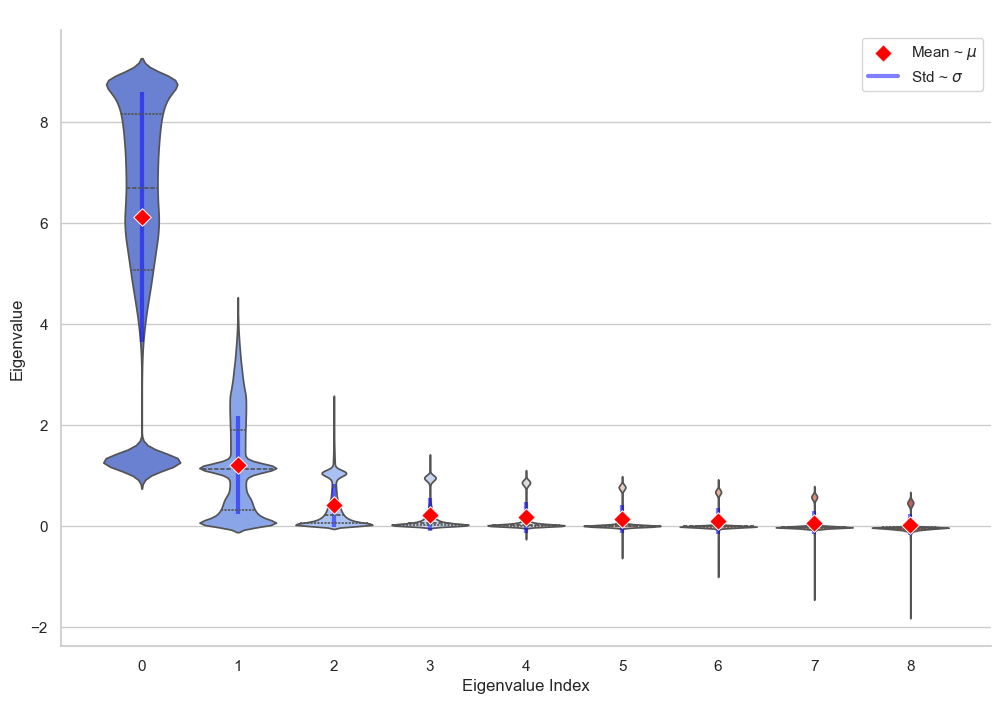
\includegraphics[width=0.5\textwidth]{figures/06_ModelExploration/1_InputData/eigval_violin_raw.png}}}
    \subfloat[]{{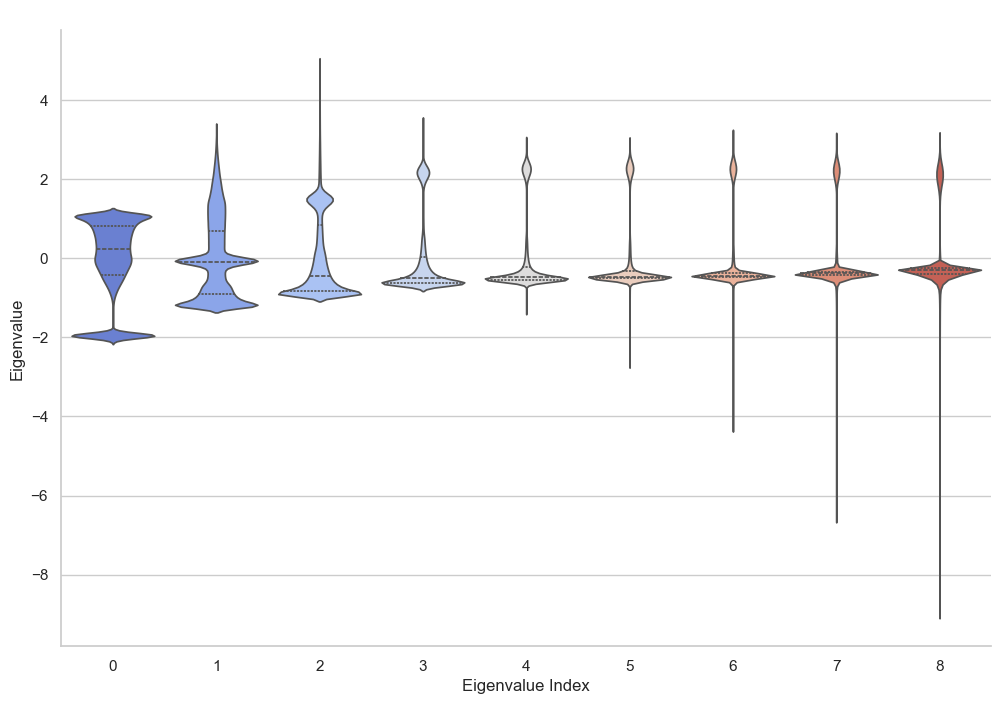
\includegraphics[width=0.5\textwidth]{figures/06_ModelExploration/1_InputData/eigval_violin_norm.png}}}
    \caption{Distributions of the eigenvalues \( \bfL \) before (a) and after (b) index-wise normalization.}
    \label{fig:eigenvalues_norm}
\end{figure}

The violin plot of the unnormalized
eigenvalues, shows that the eigenvalues, belonging noise-only scenarios, are clustered around the noise variance \( \sigma^2_{\eta} = 1\si{\micro\volt\squared}\),
and that an intuitive manual separation of the signal and noise eigenvalues is in most cases only possible for \( N < 3 \).
\hyperref[fig:eigenvalues_norm]{Figure~\ref*{fig:eigenvalues_norm}a} also depicts the mean and standard deviation of the
unnormalized eigenvalues, which additionally are gathered in \autoref{tab:dataset_stats}.

\begin{table}[H]
    \centering
    \caption{Statistics of Training Dataset Eigenvalues}
    \label{tab:dataset_stats}
    \begin{tabular}{lrrrrrrrrr}
    \toprule
    & \multicolumn{9}{c}{\textbf{Eigenvalue Index}} \\
    \cmidrule{2-10}
    & 1 & 2 & 3 & 4 & 5 & 6 & 7 & 8 & 9 \\
    \midrule
    \( \mu_i \) & 6.122 & 1.220 & 0.419 & 0.236 & 0.179 & 0.143 & 0.110 & 0.075 & 0.035 \\
    \( \sigma_i \) & 2.478 & 0.973 & 0.428 & 0.334 & 0.305 & 0.279 & 0.253 & 0.229 & 0.203 \\
    \bottomrule
    \end{tabular}
\end{table}



The evaluation of index-wise normalization's role in enhancing the predictive capabilities of an early \gls{cnn} iteration,
is detailed in \autoref{tab:model_performance}.

\begin{table}[H]
    \centering
    \caption{Impact of input data normalization on model performance}
    \label{tab:model_performance}
    \begin{tabular}{@{}lcccccc@{}}
    \toprule
    & \multicolumn{2}{c}{\( \meanLossCEVal \)} & \multicolumn{2}{c}{ \( \meanAccVal \)} & \multicolumn{2}{c}{\#MACs} \\
    \cmidrule(lr){2-3} \cmidrule(lr){4-5} \cmidrule(lr){6-7}
    Normalization & \( \nu \) & \( \%\Delta \) & \( \nu \) & \( \%\Delta \) &  &\\
    \midrule
    False & 0.616 & — & 0.725 & — &  — \\
    True & 0.615 & \gnbx{-0.30\%} & 0.726 & \gnbx{0.06\%} & \redbigoplus{} \\
    \bottomrule
    \end{tabular}
\end{table}

The results in \autoref{tab:model_performance} indicate that the index-wise normalization yields only a marginal improvement in the
model's performance, with a slight decrease in the mean validation loss%
\footnote{
    \( \meanLossVal \coloneq \mathbb{E}_{(\mbf{Z}, \mbf{Y}_N) \sim \DVal}[\lossCEVal(\mbf{Z}, \dot{\mbf{Y}}_N)]\), \( \mbf{Z} \) being
    the model's logits, and \( \dot{\mbf{Y}}_N \) the one-hot encoded ground truth labels.
}.
and a neglectable increase in the validation accuracy,
while coming at the cost of an increased number of \glspl{mac} through the additional normalization operations.


\subsubsection{Reevaluation of Index-wise Normalization}
\label{subsubsec:reevaluation_index_wise_normalization}

Upon retrospective reflection of the index-wise normalization approach, several insights have emerged that warrant
reconsideration of its appropriateness for the task at hand.

Firstly, the examination of the eigenvalue distribution underscores a relatively constrained variance, particularly
highlighted by a manageable peak to peak spread and level difference:
\begin{align*}
    \Delta\lambda_{pp} &= \max(\bfLT^{\D}_{:,:}) - \min(\bfLT^{\D}_{:,:}) \approx 11.2\si{\micro\volt\squared}, \\
    L_{\mu,pp} &= L_{\mu_1} - L_{\mu_M} = \num{44.9}\si{\decibel}.
\end{align*}

The practice of index-wise normalization, while theoretically enhancing uniformity across eigenvalue magnitudes,
amplifies the variability of lower-magnitude eigenvalues due to their low relatively low standard deviation and the
resulting inherent reciprocal scaling effect on outliers. This increased spread would mostly affect noise eigenvalues,
whose values might not encode any meaningful information about the model order, due to the effects of sub-sampling.
Enforcing uniformity across the priorities of all eigenvalues might not be aligned with the task's inherent
requirements.

Another argument advocating against normalization is the fact that the mean and standard deviation of some eigenvalues
exhibit low absolute values, which would exacerbate numerical errors in low-precision computational environments.
The subtraction of two relatively small numbers and the subsequent division by a small number would most likely lead to
the occurrence of high numerical errors, especially in the case of hardware implementation, which would require lower
precision fixed-point numbers.

Given the neglectable performance gain and the additional computational cost, the low complexity of the input data, and
the aforementioned detrimental effects, it was decided not to utilize the normalized eigenvalues as input data for the
networks.



% \section{Previous Deep Learning Approaches}
% [\cite{yang2020}]
% ```
% Based on information theory [6], the covariance matrix C contains the key information for the source number detection. One natural idea is to employ DNN to learn the source number directly from the covariance matrix C. However, it is would not be an effective way to to so due to the information redun- dancy in C that contains all unknown information besides the number of sources (will be verified in simulations).
% Although DL exhibits powerful learning capability in extracting features from massive data, model information, if can be well utilized, would provide significant enhancement in performance [11]. To see this, let us express C as

% where lambda and um are the m-th eigenvalue and correspond- ing eigenvector of C, respectively. From the array signal processing theory [5], the eigenvectors would construct the signal subspace and the noise subspace, from which the ESPRIT and MUSIC algorithms can be applied to estimate the DOA, respectively. Nevertheless, it is clearly that eigenvectors themselves do not contain information of the number of the sources and hence would bring redundancy if being input to the DNN. Hence, instead of input the whole C, we propose to only input the DNN the eigenvalues , which is also consistent with the AIC and MDL approaches. Notice that the eigenvalues  are all real numbers, therefore, complex operations are not required in the proposed ERNet and ECNet.
% ```
% They employed a fully connected NN, and no sub-sampling
% + Eigenvalues and Eigenvectors are \( \in \mathbb{R} \) and not complex such as the covariance matrix
% + \cite{yang2020} showed <überlegene> performance of eigenvalues over covariance matrix in for non-coherent sources and varying numbers of snapshots
% - \cite{yang2020} When the sources are coherent, which is the common in the real environment, the signal covariance matrix is rank- deficient, and therefore the performance of eigenvalue based methods degrades [16]. To solve the problem, the FBSS scheme is adopted [9], where the the total array of M antennas is divided forward/backward into overlapping sub-arrays with size M 0. The number of forward/backward sub-arrays is T = M - M0 + 1. Note that the M0 >     K and T >= K should be satisfied as proved in [16]. Then, the forward/backward averaged covariance matrix is given by [9]
